\frame{
\frametitle{C\'omo crear un repositorio}
 % como se crea el repositorio
\begin{enumerate}
\item Creamos el directorio  (mkdir) 
\item Desde la terminal nos ubicamos en el directorio (cd)
\item Digitamos "git init"
\end{enumerate}

Si ya habíamos creado el repositorio podemos clonarlo.Ubicados en el directorio, digitamos "git clone [URL del repositorio]".

\begin{figure}[t]
    \centering
    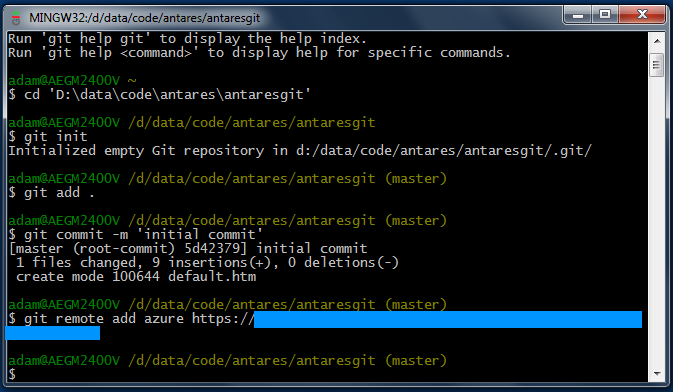
\includegraphics[width=0.5\textwidth]{Images/4}
\end{figure}
}
